\documentclass{standalone}
\usepackage{tikz}
\usetikzlibrary{patterns, positioning}
\usepackage[sfdefault]{ClearSans} %% option 'sfdefault' activates Clear Sans as the default text font
\usepackage[T1]{fontenc}

\begin{document}
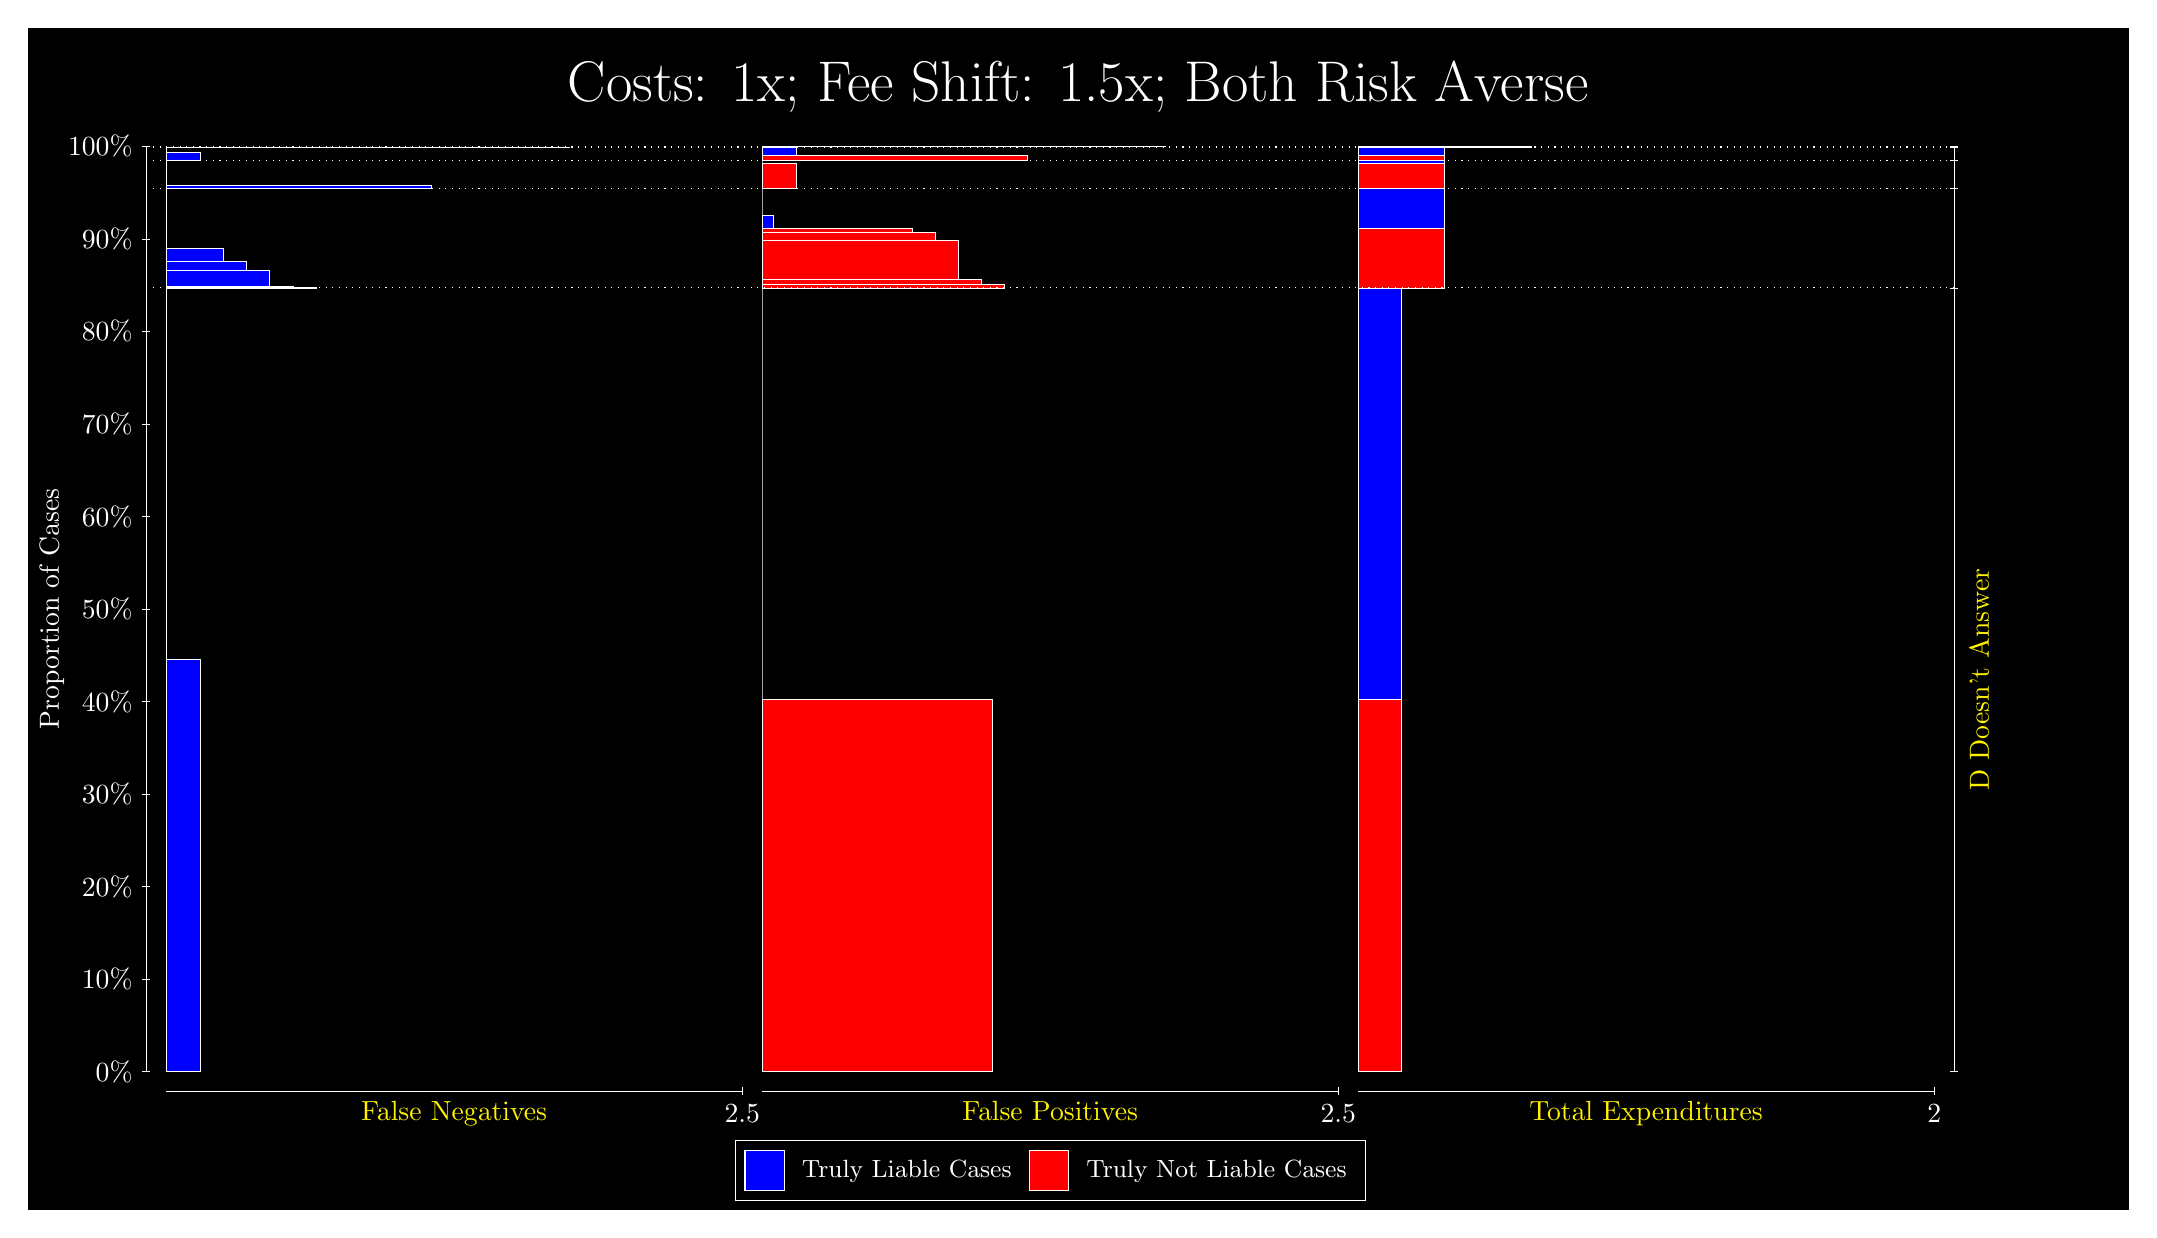
\begin{tikzpicture}
\draw[fill=black] (0,0) rectangle (26.667,15);
\draw[text=white] (0,13.5) rectangle (26.667,15) node[midway] {\huge Costs: 1x; Fee Shift: 1.5x; Both Risk Averse};
\draw[white, very thin] (1.5,1.75) -- (1.5,13.5);
\node[rotate=90, text=white, anchor=center] at (0.3, 7.625) {Proportion of Cases};
\draw[white, very thin] (1.45,1.75) -- (1.55,1.75);
\node[text=white, anchor=east] at (1.45, 1.75) {0\%};
\draw[white, very thin] (1.45,2.925) -- (1.55,2.925);
\node[text=white, anchor=east] at (1.45, 2.925) {10\%};
\draw[white, very thin] (1.45,4.1) -- (1.55,4.1);
\node[text=white, anchor=east] at (1.45, 4.1) {20\%};
\draw[white, very thin] (1.45,5.275) -- (1.55,5.275);
\node[text=white, anchor=east] at (1.45, 5.275) {30\%};
\draw[white, very thin] (1.45,6.45) -- (1.55,6.45);
\node[text=white, anchor=east] at (1.45, 6.45) {40\%};
\draw[white, very thin] (1.45,7.625) -- (1.55,7.625);
\node[text=white, anchor=east] at (1.45, 7.625) {50\%};
\draw[white, very thin] (1.45,8.8) -- (1.55,8.8);
\node[text=white, anchor=east] at (1.45, 8.8) {60\%};
\draw[white, very thin] (1.45,9.975) -- (1.55,9.975);
\node[text=white, anchor=east] at (1.45, 9.975) {70\%};
\draw[white, very thin] (1.45,11.15) -- (1.55,11.15);
\node[text=white, anchor=east] at (1.45, 11.15) {80\%};
\draw[white, very thin] (1.45,12.325) -- (1.55,12.325);
\node[text=white, anchor=east] at (1.45, 12.325) {90\%};
\draw[white, very thin] (1.45,13.5) -- (1.55,13.5);
\node[text=white, anchor=east] at (1.45, 13.5) {100\%};

\draw[white, very thin] (24.457,1.75) -- (24.457,13.5);
\draw[white, very thin] (24.407,1.75) -- (24.507,1.75);
\node[anchor=west] at (24.407, 1.75) {};
\draw[white, very thin] (24.407,11.703) -- (24.507,11.703);
\node[anchor=west] at (24.407, 11.703) {};
\draw[white, very thin] (24.407,12.967) -- (24.507,12.967);
\node[anchor=west] at (24.407, 12.967) {};
\draw[white, very thin] (24.407,13.32) -- (24.507,13.32);
\node[anchor=west] at (24.407, 13.32) {};
\draw[white, very thin] (24.407,13.488) -- (24.507,13.488);
\node[anchor=west] at (24.407, 13.488) {};
\draw[white, very thin] (24.407,13.496) -- (24.507,13.496);
\node[anchor=west] at (24.407, 13.496) {};
\draw[white, very thin] (24.407,13.5) -- (24.507,13.5);
\node[anchor=west] at (24.407, 13.5) {};

\draw[white, very thin, fill=blue] (1.75,1.75) rectangle (2.1891,6.9795);
\draw[white, very thin, fill=red] (1.75,6.9795) rectangle (1.75,11.703);
\draw[white, very thin, fill=blue] (1.75,11.703) rectangle (3.6529,11.707);
\draw[white, very thin, fill=blue] (1.75,11.707) rectangle (3.3602,11.721);
\draw[white, very thin, fill=blue] (1.75,11.721) rectangle (3.0674,11.92);
\draw[white, very thin, fill=blue] (1.75,11.92) rectangle (2.7746,12.043);
\draw[white, very thin, fill=blue] (1.75,12.043) rectangle (2.4819,12.211);
\draw[white, very thin, fill=red] (1.75,12.211) rectangle (1.75,12.967);
\draw[white, very thin, fill=blue] (1.75,12.967) rectangle (5.1167,13.002);
\draw[white, very thin, fill=red] (1.75,13.002) rectangle (1.75,13.32);
\draw[white, very thin, fill=blue] (1.75,13.32) rectangle (2.1891,13.419);
\draw[white, very thin, fill=red] (1.75,13.419) rectangle (1.75,13.488);
\draw[white, very thin, fill=blue] (1.75,13.488) rectangle (6.8732,13.49);
\draw[white, very thin, fill=red] (1.75,13.49) rectangle (1.75,13.496);
\draw[white, very thin, fill=red] (1.75,13.496) rectangle (1.75,13.498);
\draw[white, very thin, fill=blue] (1.75,13.498) rectangle (1.75,13.5);
\draw[white, very thin, fill=red] (9.3189,1.75) rectangle (12.246,6.4737);
\draw[white, very thin, fill=blue] (9.3189,6.4737) rectangle (9.3189,11.703);
\draw[white, very thin, fill=red] (9.3189,11.703) rectangle (12.393,11.744);
\draw[white, very thin, fill=red] (9.3189,11.744) rectangle (12.1,11.817);
\draw[white, very thin, fill=red] (9.3189,11.817) rectangle (11.807,12.308);
\draw[white, very thin, fill=red] (9.3189,12.308) rectangle (11.515,12.411);
\draw[white, very thin, fill=red] (9.3189,12.411) rectangle (11.222,12.46);
\draw[white, very thin, fill=blue] (9.3189,12.46) rectangle (9.4652,12.627);
\draw[white, very thin, fill=blue] (9.3189,12.627) rectangle (9.3189,12.967);
\draw[white, very thin, fill=red] (9.3189,12.967) rectangle (9.758,13.285);
\draw[white, very thin, fill=blue] (9.3189,13.285) rectangle (9.3189,13.32);
\draw[white, very thin, fill=red] (9.3189,13.32) rectangle (12.686,13.389);
\draw[white, very thin, fill=blue] (9.3189,13.389) rectangle (9.758,13.488);
\draw[white, very thin, fill=red] (9.3189,13.488) rectangle (9.3189,13.494);
\draw[white, very thin, fill=blue] (9.3189,13.494) rectangle (9.3189,13.496);
\draw[white, very thin, fill=red] (9.3189,13.496) rectangle (14.442,13.498);
\draw[white, very thin, fill=blue] (9.3189,13.498) rectangle (11.515,13.5);
\draw[white, very thin, fill=red] (16.888,1.75) rectangle (17.437,6.4737);
\draw[white, very thin, fill=blue] (16.888,6.4737) rectangle (17.437,11.703);
\draw[white, very thin, fill=red] (16.888,11.703) rectangle (17.986,12.46);
\draw[white, very thin, fill=blue] (16.888,12.46) rectangle (17.986,12.967);
\draw[white, very thin, fill=red] (16.888,12.967) rectangle (17.986,13.285);
\draw[white, very thin, fill=blue] (16.888,13.285) rectangle (17.986,13.32);
\draw[white, very thin, fill=red] (16.888,13.32) rectangle (17.986,13.389);
\draw[white, very thin, fill=blue] (16.888,13.389) rectangle (17.986,13.488);
\draw[white, very thin, fill=red] (16.888,13.488) rectangle (19.083,13.494);
\draw[white, very thin, fill=blue] (16.888,13.494) rectangle (19.083,13.496);
\draw[white, very thin, fill=red] (16.888,13.496) rectangle (19.083,13.498);
\draw[white, very thin, fill=blue] (16.888,13.498) rectangle (19.083,13.5);
\draw[white, dotted] (1.5,11.703) -- (24.457,11.703);
\draw[white, dotted] (1.5,12.967) -- (24.457,12.967);
\draw[white, dotted] (1.5,13.32) -- (24.457,13.32);
\draw[white, dotted] (1.5,13.488) -- (24.457,13.488);
\draw[white, dotted] (1.5,13.496) -- (24.457,13.496);
\draw[white, very thin] (1.75,1.5) -- (9.0689,1.5);
\node[text=yellow, anchor=north] at (5.4094, 1.5) {False Negatives};
\draw[white, very thin] (9.0689,1.45) -- (9.0689,1.55);
\node[text=white, anchor=north] at (9.0689, 1.45) {2.5};

\draw[white, very thin] (9.3189,1.5) -- (16.638,1.5);
\node[text=yellow, anchor=north] at (12.978, 1.5) {False Positives};
\draw[white, very thin] (16.638,1.45) -- (16.638,1.55);
\node[text=white, anchor=north] at (16.638, 1.45) {2.5};

\draw[white, very thin] (16.888,1.5) -- (24.207,1.5);
\node[text=yellow, anchor=north] at (20.547, 1.5) {Total Expenditures};
\draw[white, very thin] (24.207,1.45) -- (24.207,1.55);
\node[text=white, anchor=north] at (24.207, 1.45) {2};

\node[text=yellow, centered, rotate=90] at (24.777, 6.7266) {D Doesn't Answer};






\draw (12.978300999999998,1.5) node[draw=none] (baseCoordinate) {};
\begin{scope}[align=center]
        \matrix[scale=0.5, draw=white, below=0.5cm of baseCoordinate, nodes={draw}, column sep=0.1cm]{
            \node[rectangle, draw, minimum width=0.5cm, minimum height=0.5cm, fill=blue] {}; &
            \node[draw=none, font=\small, text=white] (B) {Truly Liable Cases}; &
            \node[rectangle, draw, minimum width=0.5cm, minimum height=0.5cm, fill=red] {}; &
            \node[draw=none, font=\small, text=white] (B) {Truly Not Liable Cases}; \\
            };
\end{scope}

\end{tikzpicture}
\end{document}